% ---------------------------------------------------------------------------
% Caderno 4 — Curvatura e superfície de resposta
% Murilo Miguel Narciso, Instituto Militar de Engenharia.
% Compilação (MiKTeX fora do PATH):
%   $env:PATH = "C:\Users\Narcísius\AppData\Local\Programs\MiKTeX\miktex\bin\x64;" + $env:PATH
%   pdflatex -interaction=nonstopmode -include-directory=..\estilo main.tex   (três vezes)
% ---------------------------------------------------------------------------
\documentclass{doeapostila}

% ---------------------------------------------------------------------------
% macros.tex — notação matemática comum aos cinco cadernos.
% Fixada antes de qualquer caderno começar, para os cinco não divergirem.
% Uso: % ---------------------------------------------------------------------------
% macros.tex — notação matemática comum aos cinco cadernos.
% Fixada antes de qualquer caderno começar, para os cinco não divergirem.
% Uso: % ---------------------------------------------------------------------------
% macros.tex — notação matemática comum aos cinco cadernos.
% Fixada antes de qualquer caderno começar, para os cinco não divergirem.
% Uso: \input{../estilo/macros} no preâmbulo de cada main.tex.
% ---------------------------------------------------------------------------

% Somas de quadrados
\newcommand{\SQT}{\mathrm{SQ}_{\mathrm{T}}}    % total
\newcommand{\SQR}{\mathrm{SQ}_{\mathrm{R}}}    % da regressão
\newcommand{\SQr}{\mathrm{SQ}_{\mathrm{r}}}    % residual
\newcommand{\SQfaj}{\mathrm{SQ}_{\mathrm{faj}}}% falta de ajuste
\newcommand{\SQep}{\mathrm{SQ}_{\mathrm{ep}}}  % erro puro

% Médias quadráticas: \MQ{R}, \MQ{r}, \MQ{faj}, \MQ{ep}
\newcommand{\MQ}[1]{\mathrm{MQ}_{\mathrm{#1}}}

% Coeficientes de determinação
\newcommand{\Rdois}{R^{2}}
\newcommand{\Rajus}{R^{2}_{\mathrm{aj}}}

% Efeitos: \efeito{1}, \efeito{12}
\newcommand{\efeito}[1]{E_{#1}}

% Álgebra matricial do ajuste por mínimos quadrados
\newcommand{\vetbeta}{\boldsymbol{\beta}}
\newcommand{\matX}{\mathbf{X}}
\newcommand{\vety}{\mathbf{y}}
 no preâmbulo de cada main.tex.
% ---------------------------------------------------------------------------

% Somas de quadrados
\newcommand{\SQT}{\mathrm{SQ}_{\mathrm{T}}}    % total
\newcommand{\SQR}{\mathrm{SQ}_{\mathrm{R}}}    % da regressão
\newcommand{\SQr}{\mathrm{SQ}_{\mathrm{r}}}    % residual
\newcommand{\SQfaj}{\mathrm{SQ}_{\mathrm{faj}}}% falta de ajuste
\newcommand{\SQep}{\mathrm{SQ}_{\mathrm{ep}}}  % erro puro

% Médias quadráticas: \MQ{R}, \MQ{r}, \MQ{faj}, \MQ{ep}
\newcommand{\MQ}[1]{\mathrm{MQ}_{\mathrm{#1}}}

% Coeficientes de determinação
\newcommand{\Rdois}{R^{2}}
\newcommand{\Rajus}{R^{2}_{\mathrm{aj}}}

% Efeitos: \efeito{1}, \efeito{12}
\newcommand{\efeito}[1]{E_{#1}}

% Álgebra matricial do ajuste por mínimos quadrados
\newcommand{\vetbeta}{\boldsymbol{\beta}}
\newcommand{\matX}{\mathbf{X}}
\newcommand{\vety}{\mathbf{y}}
 no preâmbulo de cada main.tex.
% ---------------------------------------------------------------------------

% Somas de quadrados
\newcommand{\SQT}{\mathrm{SQ}_{\mathrm{T}}}    % total
\newcommand{\SQR}{\mathrm{SQ}_{\mathrm{R}}}    % da regressão
\newcommand{\SQr}{\mathrm{SQ}_{\mathrm{r}}}    % residual
\newcommand{\SQfaj}{\mathrm{SQ}_{\mathrm{faj}}}% falta de ajuste
\newcommand{\SQep}{\mathrm{SQ}_{\mathrm{ep}}}  % erro puro

% Médias quadráticas: \MQ{R}, \MQ{r}, \MQ{faj}, \MQ{ep}
\newcommand{\MQ}[1]{\mathrm{MQ}_{\mathrm{#1}}}

% Coeficientes de determinação
\newcommand{\Rdois}{R^{2}}
\newcommand{\Rajus}{R^{2}_{\mathrm{aj}}}

% Efeitos: \efeito{1}, \efeito{12}
\newcommand{\efeito}[1]{E_{#1}}

% Álgebra matricial do ajuste por mínimos quadrados
\newcommand{\vetbeta}{\boldsymbol{\beta}}
\newcommand{\matX}{\mathbf{X}}
\newcommand{\vety}{\mathbf{y}}


\definecaderno{4}{Curvatura e superfície de resposta}

\graphicspath{{../figuras/out/}}

\begin{document}

\begin{center}
  {\large\bfseries Caderno 4\\Curvatura e superfície de resposta}\par\smallskip
  {\normalsize Murilo Miguel Narciso}\par\smallskip
  {\footnotesize Instituto Militar de Engenharia \textbullet{} \today}
\end{center}

\vspace{0.6\baselineskip}

\noindent
O Caderno 2 mostrou como estimar efeitos principais e interações a partir de
um planejamento fatorial em dois níveis. Esse instrumento tem um limite
estrutural: dois níveis por fator definem uma reta em cada direção, nunca uma
curva, de modo que nenhum fatorial $2^{k}$ consegue, por si só, detectar que a
resposta atinge um máximo, um mínimo ou um ponto de sela dentro da região
experimental. Este caderno percorre a solução desse problema em três etapas
que se encadeiam. O planejamento fatorial detecta a existência de curvatura,
mas não a mede: o ponto central acrescenta essa capacidade, ao custo de
confundir o efeito quadrático agregado sem dizer de qual fator ele vem. A
composição central resolve essa ambiguidade, acrescentando pontos além dos
vértices do cubo que permitem estimar cada termo quadrático individualmente.
O fio condutor do caderno é justamente essa sequência: fatorial insuficiente,
ponto central que detecta e confunde, composição central que separa.

Depois de apresentar a composição central, o caderno introduz o
planejamento de Box-Behnken como uma segunda via para o mesmo modelo de
segunda ordem, mostra como classificar o ponto ótimo de uma superfície já
ajustada em máximo, mínimo ou ponto de sela, e termina explicando por que a
plataforma que acompanha este material recomenda, na prática, uma variante
de face centrada da composição central, e não a versão rotacionável cuja
álgebra é desenvolvida ao longo do texto.

\vspace{0.6\baselineskip}

\tableofcontents

\section{O limite do planejamento em dois níveis}

Um fator investigado em apenas dois níveis, codificados $z=-1$ e $z=+1$,
fornece exatamente dois pontos por onde passar uma reta. Não há informação
suficiente para distinguir uma relação linear de uma relação com curvatura,
porque qualquer modelo de segunda ordem $y = a_{0} + a_{1}z + a_{2}z^{2}$
avaliado só nesses dois pontos é indistinguível, para fins de ajuste, de um
modelo puramente linear com intercepto ajustado. Formalmente, a coluna de
$z^{2}$ no planejamento $2^{k}$ vale sempre $1$, em ambos os níveis, e por
isso se confunde inteiramente com a coluna do intercepto: $\sum z^{2} = 2^{k}$
mas essa soma não distingue nenhuma variação de $z^{2}$ em torno de sua
própria média, porque não há variação, o valor é constante.

A consequência prática é que o planejamento fatorial $2^{k}$, por mais
réplicas que receba, nunca vai revelar se a resposta verdadeira se curva
entre os dois níveis testados. Se o fenômeno físico tiver um ótimo interior,
um máximo de resistência num teor intermediário de aditivo, por exemplo, o
fatorial em dois níveis relata dois pontos da encosta dessa colina sem nunca
enxergar o cume.

\begin{aplicacao}{Um efeito principal que esconde um máximo}
Considere um fator codificado entre $-1$ e $+1$ cuja resposta verdadeira siga
$y = 3 + 0{,}5z - 2z^{2}$, com máximo em $z=0{,}125$. Um planejamento em dois
níveis mede $y(-1) = 0{,}5$ e $y(+1) = 1{,}5$, produzindo um efeito estimado
de $1{,}0$, positivo e aparentemente linear. Nenhuma das duas observações
revela que o valor no centro, $y(0) = 3$, é maior que os dois extremos
somados. O fatorial em dois níveis não está errado quanto ao que mede, apenas
não mede o que seria preciso para localizar o máximo.
\end{aplicacao}

\section{Pontos centrais}

A saída mais simples para detectar curvatura sem abandonar a estrutura do
planejamento fatorial é acrescentar réplicas no ponto central, $z_{1} =
z_{2} = \cdots = z_{k} = 0$, mantendo os $2^{k}$ vértices do cubo como estão.
O planejamento resultante tem $N_{E} = 2^{k} + N_{R0}$ ensaios, em que
$N_{R0}$ é o número de réplicas centrais, tipicamente entre três e cinco.

O ponto central desempenha duas funções simultâneas. A primeira é fornecer
uma estimativa de erro puro independente de qualquer suposição sobre a forma
do modelo, porque todas as réplicas centrais compartilham exatamente as
mesmas condições experimentais e qualquer diferença entre elas só pode vir de
ruído. A segunda função, o assunto central deste caderno, é permitir comparar
a média observada no centro com a média prevista pelo modelo linear ajustado
aos vértices: se as duas médias coincidirem, dentro do erro experimental, o
modelo linear é adequado; se divergirem, há curvatura na superfície.

\begin{aplicacao}{Por que não replicar todos os vértices em vez de usar o centro}
Replicar os $2^{k}$ vértices duplica o esforço experimental e melhora a
precisão de cada efeito, mas não acrescenta nenhuma capacidade de detectar
curvatura, pelo argumento da Seção 1: dois níveis continuam sendo dois
níveis, por mais vezes que sejam repetidos. Um pequeno número de réplicas no
centro, em contraste, custa poucos ensaios adicionais e abre uma porta que a
réplica nos vértices nunca abriria.
\end{aplicacao}

A escolha de $N_{R0}$ dentro da faixa de três a cinco réplicas equilibra
dois interesses opostos. Poucas réplicas centrais, como o mínimo de três,
mantêm baixo o custo experimental adicional, mas deixam o erro puro com
poucos graus de liberdade, o que torna o teste de curvatura e as futuras
estimativas de variância mais instáveis: com três réplicas, o erro puro
tem apenas dois graus de liberdade, o mínimo tecnicamente utilizável, como
o exemplo da Seção 3 evidencia. Cinco réplicas centrais, no outro extremo,
fornecem quatro graus de liberdade para o erro puro, uma estimativa bem
mais estável, ao custo de dois ensaios adicionais. Entre esses dois
extremos não há um valor universalmente correto: a escolha depende do
custo relativo de cada ensaio adicional frente ao ganho de precisão na
estimativa do erro puro, uma decisão que cabe ao pesquisador e que a
plataforma deixa explicitamente configurável, em vez de fixar um único
valor padrão para todo experimento.

\section{Teste de curvatura}

Sejam $\bar{y}_{F}$ a média dos $n_{F} = 2^{k}$ pontos fatoriais e
$\bar{y}_{C}$ a média dos $n_{C} = N_{R0}$ pontos centrais. Sob um modelo
puramente linear, a previsão no centro é a própria média dos vértices, de
modo que a diferença $\bar{y}_{F} - \bar{y}_{C}$ deveria ser nula a menos de
ruído. O teste de curvatura converte essa diferença numa soma de quadrados
com um único grau de liberdade,
\begin{equation}
  SQ_{\mathrm{curv}} = \frac{n_{F}\, n_{C}\, (\bar{y}_{F} - \bar{y}_{C})^{2}}
                             {n_{F} + n_{C}} ,
  \label{eq:sqcurv}
\end{equation}
que entra na tabela de análise de variância como mais uma linha, ao lado dos
efeitos principais e interações, e é comparada ao erro puro estimado pela
variância entre as réplicas centrais, $\MQ{ep} = \sum(y_{i}-\bar{y}_{C})^{2}
/(n_{C}-1)$, por meio da razão $F = SQ_{\mathrm{curv}}/\MQ{ep}$, com
distribuição $F(1,\,n_{C}-1)$ sob a hipótese de ausência de curvatura.

A leitura do teste é direta: $p < 0{,}05$ indica que a superfície verdadeira
se afasta de um plano dentro da região estudada, e que um modelo puramente
linear vai subestimar ou superestimar sistematicamente a resposta em algum
ponto interno. Este teste está implementado na plataforma que acompanha este
material e aparece automaticamente como linha "Curvatura" na tabela de
análise de variância sempre que o planejamento tiver pontos centrais e todos
os fatores forem quantitativos.

O cálculo completo, número por número, é mais instrutivo que a fórmula
isolada. Retome o fatorial $2^{2}$ do catalisador já apresentado em
\texttt{peixoto-2x2}, com respostas de rendimento $57/61$, $92/88$, $55/53$
e $66/70$ nos quatro vértices, médias de célula $59{,}0$, $90{,}0$, $54{,}0$
e $68{,}0$, e média fatorial $\bar{y}_{F} = 67{,}75$. Como esse material
original não inclui pontos centrais, o conjunto identificado neste caderno
por \texttt{curvatura-catalisador} acrescenta três réplicas centrais
\emph{sintéticas}, geradas com semente fixa ($\mathtt{seed=42}$) a partir de
uma distribuição normal de média $78{,}0$ e desvio-padrão $\sqrt{6{,}5}$, o
mesmo nível de ruído do erro puro original do fatorial. O valor de
$78{,}0$ foi escolhido, e não medido, para simular um patamar de rendimento
mais alto no centro da faixa de temperatura e catalisador, de modo a
produzir curvatura detectável no exemplo. Este ponto é essencial: os três
valores centrais, $78{,}8$, $75{,}3$ e $79{,}9$, não correspondem a um
ensaio real do material de origem, e qualquer leitura deste exemplo precisa
preservar essa distinção entre o fatorial medido e o centro construído para
fins didáticos.

A Tabela~\ref{tab:teste-curvatura} reúne os elementos do cálculo. Com
$n_{F}=4$, $n_{C}=3$ e $\bar{y}_{F}-\bar{y}_{C} = 67{,}75-78{,}0 = -10{,}25$,
a Equação~\eqref{eq:sqcurv} fornece $SQ_{\mathrm{curv}} =
4\cdot3\cdot(-10{,}25)^{2}/7 = 180{,}1071$. O erro puro dos três centrais,
com apenas dois graus de liberdade, vale $\MQ{ep} = 5{,}77$, de modo que
$F_{0} = 180{,}1071/5{,}77 = 31{,}2144$, muito acima do quantil crítico
$F_{0{,}05}(1,2) = 18{,}5128$, com $p = 0{,}030575$.

\begin{table}[H]
  \centering
  \caption{Teste de curvatura do conjunto \texttt{curvatura-catalisador}: 2² do
    catalisador (\texttt{peixoto-2x2}) mais três pontos centrais sintéticos,
    semente 42. Fonte: \texttt{apostilas/dados/numeros.md}, chave
    \texttt{curvatura-catalisador}.}
  \label{tab:teste-curvatura}
  \begin{tabular}{l S[table-format=3.4] S[table-format=1.0]
                    S[table-format=3.4] S[table-format=2.4] S[table-format=1.6]}
    \toprule
    Fonte & {SQ} & GL & {MQ} & {$F_{0}$} & {$p$} \\
    \midrule
    Curvatura            & 180.1071 & 1 & 180.1071 & 31.2144 & 0.030575 \\
    Erro puro (centrais)  & 11.5400  & 2 & 5.7700   &         &          \\
    \bottomrule
  \end{tabular}
\end{table}

\noindent
Com $p = 0{,}031$, abaixo do limiar convencional de $5\%$, o teste rejeita a
hipótese de superfície plana mesmo com o mínimo de três réplicas centrais
utilizável na prática, o que ilustra que o teste de curvatura não exige um
grande número de réplicas para ter poder de detecção, desde que a curvatura
real seja de magnitude comparável ao ruído experimental ou maior, como
construído neste exemplo.

Detectar a curvatura, no entanto, é apenas metade do problema. O teste
desta seção responde à pergunta "existe curvatura na região estudada?",
mas não responde a "qual dos dois fatores, temperatura ou catalisador, é
responsável por ela?", nem a "o efeito quadrático de temperatura é maior
que o de catalisador?". Essas perguntas exigem um número maior de pontos
além do centro, um por eixo, o que é justamente o assunto da seção
seguinte, que mostra por que o conjunto de dados desta seção não permite
respondê-las e o que precisa ser acrescentado ao planejamento para que
passem a ser respondíveis.

\begin{aplicacao}{Lendo o resultado de um teste de curvatura significativo}
Um teste de curvatura com $p = 0{,}02$ não indica qual fator, entre vários
investigados, é responsável pela curvatura, nem qual sinal ela tem. Indica
apenas que existe, agregada sobre todos os fatores quantitativos do
planejamento, curvatura suficiente para não ser atribuída ao ruído. A Seção 4
mostra por que essa informação vem sempre agregada e nunca decomposta por
fator, quando a única fonte de pontos além dos vértices é o centro.
\end{aplicacao}

\section{O efeito quadrático confundido}

A razão pela qual o teste de curvatura não distingue entre fatores está na
estrutura de colunas do modelo. Para $k=2$, com um ponto central
acrescentado, a matriz de momentos que envolve os termos quadráticos deixa
de ser diagonal: a coluna de $z_{1}^{2}$ e a coluna de $z_{2}^{2}$, que valem
$1$ em todos os quatro vértices e $0$ no centro, são idênticas entre si em
todo o planejamento, e ambas se correlacionam com a coluna do intercepto.
Não é possível, com apenas um ponto adicional, separar quanto da curvatura
observada vem de $z_{1}^{2}$ e quanto vem de $z_{2}^{2}$: o que se estima é
uma combinação linear fixa dos dois, e não os dois coeficientes
individualmente.

A Tabela~\ref{tab:colunas-confundidas} escreve essas colunas por extenso
para o fatorial $2^{2}$ com um único ponto central, cinco ensaios ao todo.
A identidade entre a quarta e a quinta coluna, $z_{1}^{2}$ e $z_{2}^{2}$, é
visível linha a linha, e não apenas uma afirmação abstrata sobre a
estrutura do planejamento.

\begin{table}[H]
  \centering
  \caption{Colunas codificadas do fatorial $2^{2}$ com um ponto central,
    cinco ensaios: a coluna de $z_{1}^{2}$ e a de $z_{2}^{2}$ são
    idênticas em todo o planejamento.}
  \label{tab:colunas-confundidas}
  \begin{tabular}{c S[table-format=-1.0] S[table-format=-1.0]
                    S[table-format=1.0] S[table-format=1.0]}
    \toprule
    Ensaio & {$z_{1}$} & {$z_{2}$} & {$z_{1}^{2}$} & {$z_{2}^{2}$} \\
    \midrule
    1 & -1 & -1 & 1 & 1 \\
    2 &  1 & -1 & 1 & 1 \\
    3 & -1 &  1 & 1 & 1 \\
    4 &  1 &  1 & 1 & 1 \\
    5 &  0 &  0 & 0 & 0 \\
    \bottomrule
  \end{tabular}
\end{table}

\noindent
Com apenas essas cinco linhas, qualquer tentativa de estimar $a_{11}$ e
$a_{22}$ separadamente esbarra no fato de que as colunas quarta e quinta
da Tabela~\ref{tab:colunas-confundidas} são a mesma coluna repetida: a
matriz $\matX^{\top}\matX$ correspondente é singular na submatriz que
envolve esses dois termos, e o ajuste por mínimos quadrados apresentado no
Caderno 3 não tem solução única para eles. É essa singularidade, e não uma
limitação do método de estimação, que impõe o limite descrito nesta seção.

Essa confusão é resolvida algebricamente por meio da diagonalização da
matriz de momentos, que isola um único termo quadrático agregado,
$\lambda = \sum z_{1i}^{2} / (2^{k} + N_{R0})$, cujo coeficiente é estimável
mas cuja decomposição em $a_{11}$ e $a_{22}$ individuais permanece
indeterminada. A Figura \ref{fig:grade-ponto-central} ilustra essa geometria
no espaço natural e no espaço codificado para $k=2$: o ponto central ocupa
uma posição privilegiada no meio do quadrado formado pelos quatro vértices,
mas sozinho não distingue curvatura ao longo do eixo $z_{1}$ de curvatura ao
longo do eixo $z_{2}$.

\begin{figure}[H]
  \centering
  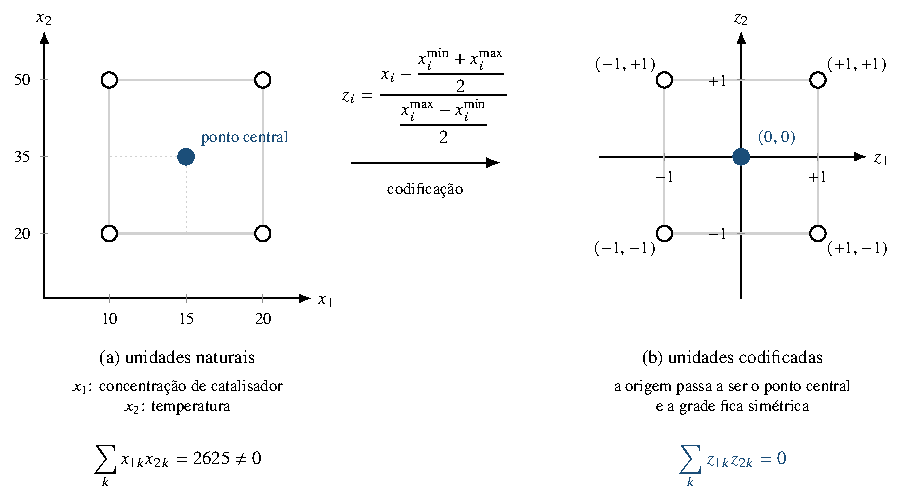
\includegraphics[width=0.72\linewidth]{c4-grade-2a2-ponto-central}
  \caption{Grade fatorial $2^{2}$ com um ponto central, representada no
    espaço natural das variáveis originais (painel a) e no espaço codificado
    $z_{1}, z_{2} \in \{-1,0,+1\}$ (painel b). O ponto central ocupa o meio
    da grade nos dois espaços, mas não fornece, por si só, informação
    separada para cada eixo.}
  \label{fig:grade-ponto-central}
\end{figure}

A saída para decompor a curvatura por fator é acrescentar mais pontos além
dos vértices, ao longo de cada eixo individualmente, o que é exatamente a
construção apresentada na Seção 7.

\section{Os quatro modelos de superfície de resposta}

Antes de introduzir a composição central, cabe situar os quatro modelos que
um planejamento de superfície de resposta pode ajustar, em ordem crescente de
complexidade. O primeiro é o modelo puramente linear nos efeitos principais,
$y = a_{0} + \sum_{j} a_{j}z_{j}$, estimável já pelo fatorial em dois níveis.
O segundo acrescenta as interações binárias, $y = a_{0} + \sum_{j} a_{j}z_{j}
+ \sum_{j<l} a_{jl}z_{j}z_{l}$, também estimável pelo fatorial completo, sem
pontos adicionais. O terceiro acrescenta apenas os termos quadráticos puros
sem interação, $y = a_{0} + \sum_{j} a_{j}z_{j} + \sum_{j} a_{jj}z_{j}^{2}$, e
o quarto, o modelo completo de segunda ordem, reúne lineares, quadráticos e
interações,
\begin{equation}
  y = a_{0} + \sum_{j} a_{j}z_{j} + \sum_{j<l} a_{jl}z_{j}z_{l}
      + \sum_{j} a_{jj}z_{j}^{2} .
  \label{eq:modelo-segunda-ordem}
\end{equation}
Os dois primeiros modelos são estimáveis por um fatorial $2^{k}$ comum; os
dois últimos exigem pontos além dos dois níveis, porque envolvem os termos
$z_{j}^{2}$ que a Seção 1 mostrou serem inestimáveis individualmente num
fatorial em dois níveis. A composição central, apresentada na Seção 7, é o
arranjo mais usado para estimar o modelo completo da Equação
\eqref{eq:modelo-segunda-ordem}.

O número de parâmetros $p$ de cada modelo, intercepto incluído, cresce na
mesma ordem: $p=1+k$ no linear, $p=1+k+\binom{k}{2}$ com interações,
$p=1+2k$ com quadráticos puros, e $p=1+2k+\binom{k}{2}$ no modelo completo
de segunda ordem. Para $k=2$, essa progressão vale $3$, $4$, $5$ e $6$
parâmetros; para $k=3$, $4$, $7$, $7$ e $10$. É esse último valor, $p=10$
para $k=3$, que fixa quantos ensaios distintos, no mínimo, qualquer
planejamento de segunda ordem precisa fornecer, patamar que tanto a
composição central quanto o Box-Behnken da Seção 8 excedem com folga, ao
custo das réplicas centrais que sustentam o erro puro.

\section{Modelo linear contra modelo com termos quadráticos}

O efeito prático de acrescentar os termos quadráticos ao modelo é mais
convincente quando visto sobre um único conjunto de dados ajustado das duas
formas. Considere nove níveis de um fator quantitativo, de $30$ a $70$ em
passos de $5$, com duas réplicas em cada nível, dezoito observações ao todo,
identificado neste material pela chave \texttt{peixoto-lin-quad}. O ajuste
linear simples e o ajuste com termo quadrático adicional produzem as
análises de variância da Tabela~\ref{tab:linear-vs-quadratico}.

\begin{table}[H]
  \centering
  \caption{Análise de variância comparada do modelo linear e do modelo com
    termo quadrático, mesmos dezoito pontos, $n=18$. Fonte: Peixoto,
    capítulo 5, p. 32 a 34.}
  \label{tab:linear-vs-quadratico}
  \begin{tabular}{l S[table-format=4.4] c S[table-format=4.4]
                    S[table-format=4.4] c S[table-format=4.4]}
    \toprule
    & \multicolumn{3}{c}{Modelo linear} & \multicolumn{3}{c}{Modelo quadrático} \\
    \cmidrule(lr){2-4}\cmidrule(lr){5-7}
    Fonte & {SQ} & GL & {MQ} & {SQ} & GL & {MQ} \\
    \midrule
    Regressão      & 6946.4083 & 1 & 6946.4083 & 8871.5924 & 2 & 4435.7962 \\
    Falta de ajuste & 1938.5917 & 7 & 276.9417  & 13.3952   & 6 & 2.2325 \\
    Erro puro       & 45.0000   & 9 & 5.0000    & 45.0000   & 9 & 5.0000 \\
    \bottomrule
  \end{tabular}
\end{table}

\noindent
Duas leituras se impõem. A primeira é que $\Rdois$ salta de $0{,}777873$,
no modelo linear, para $0{,}993459$, no modelo quadrático: quase toda a
variação que o modelo linear deixava sem explicar era, na verdade,
curvatura sistemática, não ruído. A segunda leitura, mais importante, é que
o erro puro, $45{,}0000$ com $9$ graus de liberdade nos dois casos, é
\emph{idêntico} entre os dois modelos. Isso não é coincidência: o erro puro
é propriedade exclusiva das réplicas, ou seja, dos dados, e não muda quando
se troca o modelo ajustado a eles. O que muda é a falta de ajuste, que cai de
$MQ_{\mathrm{faj}} = 276{,}9417$ para $2{,}2325$, e com ela a razão
$\MQ{faj}/\MQ{ep}$, de $55{,}39$ para $0{,}45$: o modelo linear apresenta
falta de ajuste catastrófica, muitas vezes maior que o erro experimental, e o
modelo quadrático não apresenta falta de ajuste alguma, sua razão fica bem
abaixo do valor crítico de $F$.

A Figura \ref{fig:linear-vs-quadratico} exibe as duas curvas ajustadas sobre
os mesmos pontos, tornando visualmente óbvio o que a tabela já mostrava
numericamente: a reta atravessa a nuvem de pontos sistematicamente abaixo no
meio e acima nas pontas, enquanto a parábola acompanha a curvatura real dos
dados.

\begin{figure}[H]
  \centering
  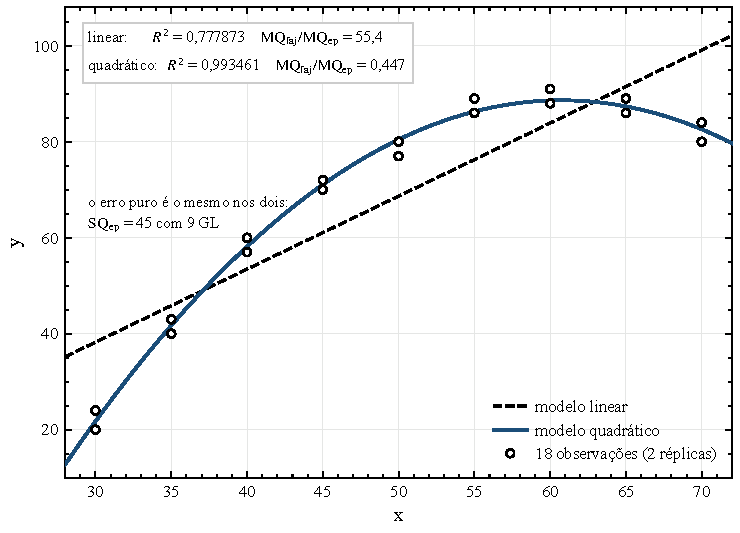
\includegraphics[width=0.85\linewidth]{c4-linear-vs-quadratico}
  \caption{Ajuste linear e ajuste quadrático sobre o mesmo conjunto de
    dezoito observações. A reta deixa um padrão sistemático nos resíduos;
    a parábola não.}
  \label{fig:linear-vs-quadratico}
\end{figure}

\begin{aplicacao}{Por que o erro puro é o mesmo nos dois modelos}
O erro puro mede quanto duas réplicas do mesmo ponto experimental diferem
entre si. Essa quantidade depende exclusivamente de quantas vezes cada ponto
foi repetido e de quanto ruído o processo físico ou de medição introduziu,
nunca de qual equação foi ajustada aos dados depois. Trocar um modelo linear
por um modelo quadrático muda a falta de ajuste, porque muda o quão bem a
curva se aproxima da média de cada ponto, mas não pode mudar a dispersão
entre réplicas do mesmo ponto, que já estava fixada antes de qualquer ajuste
ser tentado.
\end{aplicacao}

\section{Planejamento composto central}

A composição central, também chamada de planejamento composto central ou
CCD, resolve o problema de estimabilidade individual dos termos quadráticos
descrito na Seção 4, acrescentando ao fatorial em dois níveis, além dos
pontos centrais, um par de pontos axiais por fator, situados a uma distância
$\alpha$ do centro ao longo de cada eixo isoladamente, com os demais fatores
mantidos no nível central. Para $k$ fatores, o planejamento reúne $2^{k}$
pontos fatoriais, $2k$ pontos axiais e $N_{R0}$ pontos centrais,
\begin{equation}
  N_{E} = 2^{k} + 2k + N_{R0} .
  \label{eq:ne-ccd}
\end{equation}
Para $k=2$ e três réplicas centrais, isso significa $4+4+3=11$ ensaios; para
$k=3$, $8+6+N_{R0}$ ensaios.

Cada ponto axial varia apenas um fator por vez, dos $2k$ pontos totais, o que
permite estimar o coeficiente quadrático de cada fator de forma independente
dos demais, resolvendo exatamente a confusão descrita na Seção 4: com pontos
além do centro ao longo de cada eixo isolado, a matriz de momentos volta a
ser suficientemente rica para separar $a_{11}$ de $a_{22}$.

O valor de $\alpha$ é escolhido para que o planejamento tenha uma propriedade
chamada rotabilidade, segundo a qual a variância da resposta prevista depende
apenas da distância ao centro, não da direção. Essa escolha corresponde a
\begin{equation}
  \alpha = (2^{k})^{1/4} .
  \label{eq:alpha-rotavel}
\end{equation}
Para $k=2$, $\alpha = 4^{1/4} = \sqrt{2} \approx 1{,}41421$; para $k=3$,
$\alpha = 8^{1/4} \approx 1{,}68179$.

De onde vem essa quarta raiz merece ser demonstrado, e não apenas
enunciado. A variância da resposta prevista num modelo de segunda ordem
depende dos momentos da matriz de planejamento até a quarta ordem. Um
planejamento de superfície de resposta é rotacionável quando, para
quaisquer dois fatores $i \neq l$, os momentos de quarta ordem satisfazem
\begin{equation}
  \sum_{u} z_{iu}^{4} = 3 \sum_{u} z_{iu}^{2} z_{lu}^{2} ,
  \label{eq:condicao-rotabilidade}
\end{equation}
em que o somatório percorre todos os $N_{E}$ ensaios do planejamento. Essa
condição garante que a superfície de variância de previsão seja uma esfera
em torno do centro, em vez de um elipsoide alongado em alguma direção
preferencial. Nos pontos centrais, $z_{i}=z_{l}=0$, e por isso eles não
contribuem para nenhum dos dois lados da Equação
\eqref{eq:condicao-rotabilidade}; o cálculo recai inteiramente sobre os
$2^{k}$ pontos fatoriais e os $2k$ pontos axiais.

Do lado direito, $\sum_{u} z_{iu}^{2}z_{lu}^{2}$, apenas os pontos fatoriais
contribuem, porque cada ponto axial tem $z_{l}=0$ para todo fator $l$
diferente daquele que ele varia. Como $z_{iu}^{2}=z_{lu}^{2}=1$ em cada um
dos $2^{k}$ vértices do cubo, $\sum_{u} z_{iu}^{2}z_{lu}^{2} = 2^{k}$. Do
lado esquerdo, $\sum_{u} z_{iu}^{4}$, os $2^{k}$ pontos fatoriais
contribuem $2^{k}$, porque $z_{iu}^{4}=1$ em cada vértice, e os dois pontos
axiais sobre o próprio eixo $i$, situados em $z_{i}=\pm\alpha$, contribuem
$2\alpha^{4}$; os $2(k-1)$ pontos axiais dos demais eixos têm $z_{i}=0$ e
não contribuem. Logo $\sum_{u} z_{iu}^{4} = 2^{k} + 2\alpha^{4}$. Substituindo
os dois lados na Equação \eqref{eq:condicao-rotabilidade},
\begin{equation}
  2^{k} + 2\alpha^{4} = 3 \cdot 2^{k}
  \quad\Longrightarrow\quad
  2\alpha^{4} = 2\cdot 2^{k}
  \quad\Longrightarrow\quad
  \alpha^{4} = 2^{k} ,
\end{equation}
que é exatamente a Equação \eqref{eq:alpha-rotavel}. A quarta raiz não é uma
convenção arbitrária: é a única distância axial que faz o quarto momento ao
longo de cada eixo coincidir com três vezes o produto cruzado de momentos
entre eixos, condição que, por sua vez, é a que torna a variância de
previsão simétrica em relação à direção a partir do centro. Afastar os
pontos axiais além dessa distância alonga a variância de previsão ao longo
dos eixos; aproximá-los demais alonga a variância na direção diagonal entre
eixos.

\begin{aplicacao}{Conferindo a condição de rotabilidade para $k=2$}
Com $k=2$ e $\alpha=\sqrt{2}$, de modo que $\alpha^{2}=2$ e $\alpha^{4}=4$,
os três momentos da Equação \eqref{eq:condicao-rotabilidade} valem
$\sum z_{1}^{2}z_{2}^{2} = 2^{2} = 4$, apenas dos quatro pontos fatoriais, e
$\sum z_{1}^{4} = 2^{2} + 2\cdot 4 = 4 + 8 = 12$, dos quatro pontos
fatoriais mais os dois pontos axiais sobre o eixo $z_{1}$. A condição de
rotabilidade exige $\sum z_{1}^{4} = 3\sum z_{1}^{2}z_{2}^{2}$, e de fato
$12 = 3 \times 4$: a igualdade se verifica exatamente, confirmando que
$\alpha=\sqrt{2}$ é o único valor que rotaciona o planejamento para
$k=2$, não uma aproximação.
\end{aplicacao}

A leitura geométrica dessa condição é mais intuitiva do que a álgebra
sugere. Fixada a distância ao centro, a variância da resposta prevista
traça, para cada direção de saída a partir da origem, um valor específico;
reunindo essas variâncias para todas as direções a uma mesma distância,
obtém-se uma curva de nível da variância de previsão. Quando a condição de
rotabilidade é satisfeita, essa curva é exatamente uma circunferência,
para qualquer distância ao centro escolhida; quando não é satisfeita, a
curva se deforma num oval alongado ao longo dos eixos originais ou ao
longo das diagonais entre eles, dependendo de $\alpha$ estar abaixo ou
acima do valor rotacionável. Isso não significa que um planejamento não
rotacionável seja inválido, apenas que a precisão da previsão deixa de ser
uniforme com a direção, o que é aceitável quando outra restrição, como o
limite físico do laboratório discutido na Seção 11, pesa mais que essa
uniformidade.

A Figura \ref{fig:composicao-central} mostra a geometria resultante
para $k=2$: um quadrado de vértices em $(\pm1,\pm1)$, quatro pontos axiais
sobre os eixos a distância $\alpha$ do centro, e as réplicas centrais na
origem.

\begin{figure}[H]
  \centering
  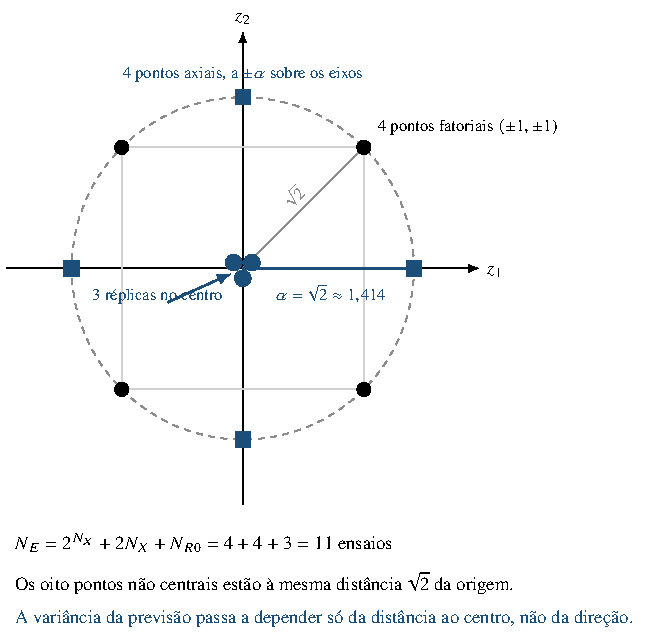
\includegraphics[width=0.68\linewidth]{c4-composicao-central}
  \caption{Geometria da composição central rotacionável para $k=2$: quatro
    pontos fatoriais nos vértices do quadrado, quatro pontos axiais a
    distância $\alpha=\sqrt{2}$ do centro ao longo de cada eixo, e réplicas
    centrais na origem.}
  \label{fig:composicao-central}
\end{figure}

Quando a execução do planejamento se estende por mais de uma sessão de
laboratório, é comum blocar o CCD em duas etapas: o primeiro bloco reúne os
pontos fatoriais e uma parte das réplicas centrais, o segundo bloco reúne os
pontos axiais e o restante das réplicas centrais. Essa divisão, se orientada
corretamente, mantém o bloco ortogonal aos efeitos de interesse, de modo que
uma eventual diferença sistemática entre as duas sessões não contamine as
estimativas dos coeficientes do fator. O exemplo da Seção 10 emprega
exatamente essa estratégia.

\begin{aplicacao}{Contagem de ensaios de uma composição central com dois fatores}
Para $k=2$ e $N_{R0}=3$, a Equação \eqref{eq:ne-ccd} fornece $N_{E} = 4 + 4 +
3 = 11$ ensaios, exatamente a estrutura empregada no estudo de caso de
solo-fibra-cimento retomado no Caderno 5: quatro combinações de vértice entre
teor de cimento e teor de fibra, quatro pontos axiais que testam cada fator
isoladamente além da faixa fatorial, e três réplicas no centro que fornecem
tanto o teste de curvatura quanto o erro puro do modelo final.
\end{aplicacao}

\section{Planejamento de Box-Behnken}

O planejamento de Box-Behnken é uma alternativa à composição central para
estimar o modelo completo de segunda ordem, distinta na geometria dos pontos
escolhidos. Em vez de combinar os vértices do cubo com pontos axiais que se
projetam para além da faixa fatorial original, o Box-Behnken posiciona seus
pontos nos pontos médios das arestas do cubo, mais réplicas centrais, sem
nunca visitar um vértice nem se afastar além dos limites $\pm1$ da faixa
codificada original.

Para três fatores, a construção resulta em doze combinações mais os pontos
centrais: cada par de fatores é variado nos quatro cantos $(\pm1,\pm1)$ com
o terceiro fator fixado no nível central, e essa operação se repete para os
três pares possíveis entre os fatores $z_{1}$, $z_{2}$ e $z_{3}$, o que
produz $3 \times 4 = 12$ combinações. A Tabela~\ref{tab:box-behnken-k3}
escreve por extenso o arranjo completo, com três réplicas centrais
acrescentadas ao final, conferido linha a linha contra a saída de
\texttt{bbdesign(3)} da biblioteca pyDOE3 1.6.2, o gerador de planejamentos
adotado pela plataforma.

\begin{table}[H]
  \centering
  \caption{Planejamento de Box-Behnken para $k=3$ fatores, $15$ ensaios:
    doze combinações nos pontos médios das arestas do cubo mais três
    réplicas centrais. Conferido contra \texttt{pyDOE3.bbdesign(3)}, versão
    1.6.2.}
  \label{tab:box-behnken-k3}
  \begin{tabular}{c S[table-format=-1.0] S[table-format=-1.0] S[table-format=-1.0]}
    \toprule
    Ensaio & {$z_{1}$} & {$z_{2}$} & {$z_{3}$} \\
    \midrule
    1  & -1 & -1 &  0 \\
    2  & -1 &  1 &  0 \\
    3  &  1 & -1 &  0 \\
    4  &  1 &  1 &  0 \\
    5  & -1 &  0 & -1 \\
    6  & -1 &  0 &  1 \\
    7  &  1 &  0 & -1 \\
    8  &  1 &  0 &  1 \\
    9  &  0 & -1 & -1 \\
    10 &  0 & -1 &  1 \\
    11 &  0 &  1 & -1 \\
    12 &  0 &  1 &  1 \\
    13 &  0 &  0 &  0 \\
    14 &  0 &  0 &  0 \\
    15 &  0 &  0 &  0 \\
    \bottomrule
  \end{tabular}
\end{table}

\noindent
Os ensaios 1 a 4 variam $z_{1}$ e $z_{2}$ nos quatro cantos, com $z_{3}$
fixo no centro; os ensaios 5 a 8 repetem a operação para $z_{1}$ e $z_{3}$,
com $z_{2}$ no centro; os ensaios 9 a 12, para $z_{2}$ e $z_{3}$, com
$z_{1}$ no centro. Generalizando para $k$ fatores, cada um dos
$\binom{k}{2}$ pares contribui quatro ensaios, de modo que o total de
ensaios do Box-Behnken é $4\binom{k}{2} + N_{R0}$, distinto da contagem
$2^{k}+2k+N_{R0}$ da composição central.

\begin{aplicacao}{Comparando o número de ensaios para três fatores}
Para $k=3$ e três réplicas centrais, a composição central da
Equação \eqref{eq:ne-ccd} exige $2^{3}+2\cdot3+3 = 8+6+3=17$ ensaios,
enquanto o Box-Behnken da Tabela~\ref{tab:box-behnken-k3} exige
$4\binom{3}{2}+3 = 12+3=15$: dois ensaios a menos, pela ausência dos
pontos axiais. A parte que cresce mais depressa com $k$ é, em cada
planejamento, diferente: a composição central acrescenta $2^{k}$ pontos
fatoriais, de crescimento exponencial, enquanto o Box-Behnken acrescenta
$4\binom{k}{2}$ pontos de aresta, de crescimento apenas quadrático. Para
$k$ pequeno a diferença é modesta, como neste exemplo com $k=3$; para $k$
grande, o crescimento exponencial da parte fatorial da composição central
acaba dominando, e a economia do Box-Behnken se torna substancial.
\end{aplicacao}

Essa diferença geométrica tem uma consequência prática direta: nenhum ponto
do Box-Behnken combina dois fatores simultaneamente em seus extremos, o que
o torna preferível quando as combinações extremas de dois ou mais fatores
são fisicamente inviáveis, perigosas ou destrutivas para o material sob
ensaio. Um exemplo típico é um processo em que temperatura máxima e pressão
máxima simultâneas excedem a capacidade do equipamento ou destroem a amostra
antes de qualquer leitura ser possível: a composição central exigiria
justamente esse ponto extremo, num de seus vértices fatoriais, enquanto o
Box-Behnken jamais o solicita.

Em contrapartida, por não incluir os vértices do cubo, o Box-Behnken
investiga uma região ligeiramente menor que a composição central para o
mesmo intervalo de fatores, e não é indicado quando a informação nos
vértices, onde interações de segunda ordem costumam se manifestar com maior
intensidade, é de particular interesse.

Quanto à propriedade de rotabilidade discutida na Seção 7 para a composição
central, o Box-Behnken não a satisfaz de forma exata para $k=3$, pela
mesma condição da Equação \eqref{eq:condicao-rotabilidade}: a distribuição
dos pontos de aresta não produz precisamente $\sum z_{i}^{4} = 3\sum
z_{i}^{2}z_{l}^{2}$. Na prática, o desvio é pequeno o suficiente para que o
planejamento seja descrito como quase rotacionável, e a diferença raramente
é perceptível na análise de uma superfície real, ao contrário do desvio
grande que a composição central de face centrada assume deliberadamente,
discutido na Seção 11.

\section{Leitura da superfície}

Uma vez ajustado o modelo completo de segunda ordem da Equação
\eqref{eq:modelo-segunda-ordem}, a superfície de resposta pode ser
visualizada de duas formas complementares: como superfície tridimensional,
que mostra a altura da resposta prevista sobre o plano dos dois fatores, e
como gráfico de contorno, que representa a mesma informação por meio de
curvas de nível, mais fácil de ler com precisão numérica e de sobrepor ao
ponto ótimo localizado. A Figura \ref{fig:superficie-plana-vs-curva} contrasta
uma superfície sem curvatura, um plano inclinado sem máximo nem mínimo
interior, com uma superfície com curvatura suficiente para apresentar um
ponto estacionário dentro da região experimental.

\begin{figure}[H]
  \centering
  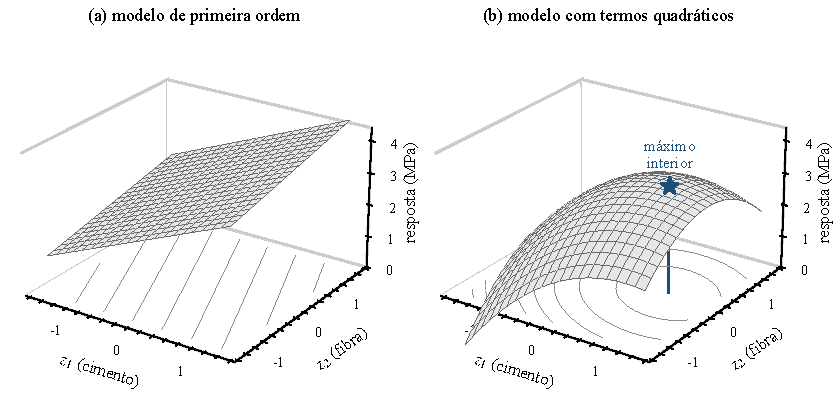
\includegraphics[width=0.92\linewidth]{c4-superficie-plana-vs-curva}
  \caption{Superfície plana, ajustada por um modelo puramente linear (painel
    a), contra superfície curva, ajustada por um modelo completo de segunda
    ordem (painel b). Somente a segunda apresenta um ponto de máximo
    interior à região experimental.}
  \label{fig:superficie-plana-vs-curva}
\end{figure}

A natureza do ponto estacionário, seja ele máximo, mínimo ou ponto de sela,
é determinada pelos autovalores da matriz de segundas derivadas do modelo
ajustado em relação aos fatores codificados. Autovalores todos negativos
indicam máximo; todos positivos indicam mínimo; sinais mistos indicam ponto
de sela, uma direção de subida e outra de descida a partir do mesmo ponto
estacionário, situação que exige inspeção cuidadosa antes de qualquer
recomendação prática ser extraída do ajuste.

Antes de classificar o ponto estacionário, é preciso localizá-lo, e essa
localização também decorre de um cálculo fechado. Para dois fatores, o
gradiente do modelo completo da Equação \eqref{eq:modelo-segunda-ordem} em
relação a $z_{1}$ e $z_{2}$ anula-se quando
\begin{equation}
  a_{1} + 2a_{11}z_{1} + a_{12}z_{2} = 0 , \qquad
  a_{2} + a_{12}z_{1} + 2a_{22}z_{2} = 0 ,
  \label{eq:gradiente-nulo}
\end{equation}
sistema que se escreve, em forma matricial, como $\mathbf{H}z^{*} = -\mathbf{a}$,
com $\mathbf{H}$ a matriz de segundas derivadas
\begin{equation}
  \mathbf{H} = \begin{bmatrix} 2a_{11} & a_{12} \\ a_{12} & 2a_{22} \end{bmatrix} ,
  \label{eq:hessiana}
\end{equation}
constante em toda a região experimental, porque o modelo é de segunda ordem
e suas derivadas de ordem superior se anulam, e $\mathbf{a}=(a_{1},a_{2})^{\top}$
o vetor dos coeficientes lineares. Sempre que $\mathbf{H}$ é inversível, o
ponto estacionário fecha-se em
\begin{equation}
  z^{*} = -\mathbf{H}^{-1}\mathbf{a} .
  \label{eq:ponto-estacionario}
\end{equation}
Uma vez localizado $z^{*}$, o sinal dos dois autovalores da mesma matriz
$\mathbf{H}$, e não o sinal isolado de $a_{11}$ e $a_{22}$, decide a
natureza desse ponto, precisamente porque o termo de interação $a_{12}$
pode inclinar a curvatura numa direção diagonal não alinhada com nenhum dos
dois eixos originais.

\begin{aplicacao}{Localizando e classificando um ponto estacionário hipotético}
Considere, a título de ilustração puramente algébrica e sem relação com
nenhum conjunto de dados deste caderno, um modelo de segunda ordem
hipotético com dois fatores, coeficientes lineares $a_{1}=a_{2}=7$ e
quadráticos $a_{11}=a_{22}=-5$, $a_{12}=-4$. A matriz de segundas
derivadas correspondente é $\mathbf{H}_{1} =
\left[\begin{smallmatrix} -10 & -4 \\ -4 & -10 \end{smallmatrix}\right]$,
com determinante $84$ e inversa
$\mathbf{H}_{1}^{-1} = \tfrac{1}{84}\left[\begin{smallmatrix} -10 & 4 \\ 4 &
-10 \end{smallmatrix}\right]$. Pela Equação \eqref{eq:ponto-estacionario},
$z^{*} = -\mathbf{H}_{1}^{-1}(7,7)^{\top} = (0{,}5,\ 0{,}5)$, um ponto
interior à região codificada usual $[-1,+1]^{2}$.

Os autovalores de $\mathbf{H}_{1}$ resolvem-se pela forma fechada de uma
matriz simétrica $2\times2$ com diagonal igual, $\lambda = a \pm b$ para
$\mathbf{H}=\left[\begin{smallmatrix}a&b\\b&a\end{smallmatrix}\right]$, o
que fornece $\lambda_{1} = -10+4=-6$ e $\lambda_{2}=-10-4=-14$: ambos
negativos, logo $z^{*}=(0{,}5,\ 0{,}5)$ é um ponto de máximo, ainda que
$a_{12}$ seja apreciável diante de $a_{11}$ e $a_{22}$.

Para contraste, considere a matriz hessiana hipotética $\mathbf{H}_{2} =
\left[\begin{smallmatrix} 8 & 6 \\ 6 & -8 \end{smallmatrix}\right]$,
correspondente a $a_{11}=4$, $a_{22}=-4$, $a_{12}=6$. Essa matriz tem traço
nulo e determinante $8\cdot(-8)-6^{2} = -100$, de modo que seus autovalores
resolvem a equação característica $\lambda^{2} - 100 = 0$, ou seja
$\lambda = \pm10$: um positivo e um negativo, logo qualquer ponto
estacionário associado a $\mathbf{H}_{2}$ seria um ponto de sela. Note-se
que, isoladamente, $a_{11}=4>0$ sugeriria mínimo ao longo de $z_{1}$ e
$a_{22}=-4<0$ sugeriria máximo ao longo de $z_{2}$; só o cálculo dos
autovalores da matriz completa resolve corretamente essa aparente
contradição.
\end{aplicacao}

Num ponto de sela, os autovetores associados a cada autovalor indicam as
direções relevantes de deslocamento a partir do ponto estacionário: ao
longo do autovetor de autovalor positivo, a resposta cresce nos dois
sentidos a partir do ponto; ao longo do autovetor de autovalor negativo,
decresce. Essa decomposição, chamada análise canônica na literatura de
superfície de resposta, é o que permite recomendar, diante de um ponto de
sela, um deslocamento ao longo da direção de autovalor positivo em busca
de valores mais altos da resposta, em vez de recomendar o próprio ponto de
sela como se fosse um ótimo, erro que a leitura isolada de $a_{11}$ e
$a_{22}$ facilmente induziria.

O exemplo de aplicação da Seção 10 emprega, no relatório de origem, um
modelo apenas com termos lineares e de bloco, sem termos quadráticos; a
matriz $\mathbf{H}$ da Equação \eqref{eq:hessiana} não se aplica a ele tal
como ajustado. É exatamente por isso que a falta de ajuste significativa
relatada naquele exemplo motiva reajustar o modelo com os termos
quadráticos completos, e é sobre esse modelo reajustado, não sobre o
modelo linear original, que a análise de autovalores desta seção deveria
ser aplicada antes de declarar um ponto ótimo.

\section{Exemplo de aplicação: a composição central com dois blocos}

O conjunto identificado neste material como \texttt{origin-ccd} reúne uma
composição central com $k=2$ fatores, teor de fibra e teor de cimento,
distribuída em dois blocos de execução, quatorze ensaios ao todo. O modelo
ajustado inclui um termo de bloco além dos dois fatores, e a
Tabela~\ref{tab:ccd-blocos} sintetiza a análise de variância completa.

\begin{table}[H]
  \centering
  \caption{Análise de variância da composição central com dois blocos.
    Fonte: relatório OriginPro, \emph{Doe Analysis pra superfície de
    resposta.pdf}.}
  \label{tab:ccd-blocos}
  \begin{tabular}{l S[table-format=3.5] c S[table-format=3.5]
                    S[table-format=1.5] S[table-format=1.5]}
    \toprule
    Fonte & {SQ} & GL & {MQ} & {$F$} & {$p$} \\
    \midrule
    Blocos            & 8.64286   & 1 & 8.64286   & 0.21681 & 0.65146 \\
    Teor de fibra      & 196.28731 & 1 & 196.28731 & 4.92385 & 0.05078 \\
    Teor de cimento    & 123.92399 & 1 & 123.92399 & 3.10862 & 0.10835 \\
    Falta de ajuste    & 361.31250 & 6 & 60.21875  & 6.45201 & 0.04628 \\
    Erro puro          & 37.33333  & 4 & 9.33333   &         &         \\
    \midrule
    Total              & 727.50000 & 13 &          &         &         \\
    \bottomrule
  \end{tabular}
\end{table}

\noindent
O erro puro tem apenas quatro graus de liberdade, resultado de dois grupos de
três réplicas centrais, um por bloco, $(3-1)+(3-1)=4$: a blocagem, embora
necessária para acomodar a execução em duas sessões, reduz o número de
réplicas centrais disponíveis para estimar o erro puro em cada bloco
isoladamente. O resultado mais relevante desta tabela é a falta de ajuste,
significativa a $p=0{,}046$, abaixo do limiar convencional de $0{,}05$. Essa
significância indica que o modelo ajustado, que neste relatório inclui
apenas termos lineares e o termo de bloco, não descreve adequadamente a
resposta: existe curvatura sistemática que o modelo linear não captura, e o
diagnóstico correto diante desse resultado é acrescentar os termos
quadráticos ao modelo, exatamente o argumento desenvolvido na Seção 6 com o
conjunto \texttt{peixoto-lin-quad}. A Figura \ref{fig:contorno-otimo}
apresenta o contorno da superfície ajustada com os termos quadráticos
completos sobre este mesmo tipo de dados, com o ponto ótimo destacado.

\begin{figure}[H]
  \centering
  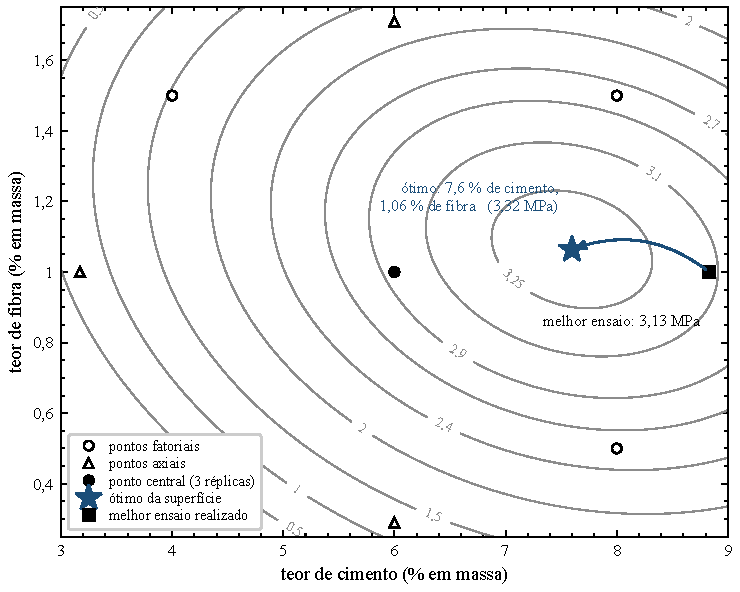
\includegraphics[width=0.72\linewidth]{c4-contorno-otimo}
  \caption{Gráfico de contorno de uma superfície de resposta ajustada com
    termos quadráticos completos, com o ponto ótimo assinalado.}
  \label{fig:contorno-otimo}
\end{figure}

\noindent
Um comentário final de reprodutibilidade numérica: o relatório de origem
desta análise emprega $\alpha=1{,}414$, uma versão truncada de $\sqrt{2}$,
enquanto a Equação \eqref{eq:alpha-rotavel} deste caderno emprega o valor
exato. A diferença entre os dois é da ordem de $10^{-6}$ nas coordenadas
axiais e não tem efeito prático sobre nenhuma conclusão deste exemplo.

\section{A escolha da plataforma: composição central de face centrada}

Todo o conteúdo deste caderno depende de uma condição simples de declarar
num fator: ele precisa ser investigado em pelo menos três níveis
codificados, $-1$, $0$ e $+1$, e não apenas nos dois extremos do fatorial.
É exatamente essa terceira coordenada que habilita, na plataforma que
acompanha este material, a construção tanto da composição central de face
centrada quanto do Box-Behnken, os dois arranjos deste caderno que estimam
o modelo completo de segunda ordem sem pedir ao pesquisador nenhum ponto
fora do intervalo físico que ele próprio declarou.

Essa última cláusula é o motivo pelo qual a plataforma recomenda, por
padrão, a composição central de face centrada, com $\alpha=1$, e não a
composição central rotacionável derivada na Seção 7. A rotabilidade exige
$\alpha=(2^{k})^{1/4}$, que vale $\sqrt{2}\approx1{,}41421$ para $k=2$ e
$8^{1/4}\approx1{,}68179$ para $k=3$: em ambos os casos, um valor maior que
$1$, o que desloca os pontos axiais para além da faixa $[-1,+1]$ que o
pesquisador declarou como o intervalo de interesse de cada fator. Essa
faixa raramente é uma escolha arbitrária; ela costuma corresponder ao
limite físico do equipamento de laboratório, à capacidade máxima segura de
um forno ou de uma prensa, ou à quantidade de material disponível para o
ensaio, de modo que solicitar um ponto além dela pode ser tecnicamente
inviável e não apenas indesejável. A composição central de face centrada,
ao fixar $\alpha=1$, posiciona os pontos axiais exatamente sobre as faces
do cubo fatorial, dentro do intervalo já declarado, e por isso nunca exige
do pesquisador uma condição que ele não possa executar.

\begin{aplicacao}{Por que o rotacionável extrapolaria a faixa do laboratório}
Considere, a título de ilustração numérica, um fator temperatura declarado
entre $150\,^{\circ}\mathrm{C}$ e $200\,^{\circ}\mathrm{C}$, faixa que
corresponde ao centro em $175\,^{\circ}\mathrm{C}$ e meia amplitude de
$25\,^{\circ}\mathrm{C}$ por unidade codificada. Um ponto axial
rotacionável, a $\alpha=1{,}41421$ unidades codificadas do centro,
corresponderia a $175 \pm 1{,}41421 \times 25 = 175\pm35{,}36\,^{\circ}
\mathrm{C}$, ou seja, um ensaio a $139{,}64\,^{\circ}\mathrm{C}$ e outro a
$210{,}36\,^{\circ}\mathrm{C}$: ambos fora do intervalo $[150,200]$ que o
pesquisador declarou, o segundo eventualmente acima do limite seguro do
forno. O ponto axial de face centrada, em contraste, com $\alpha=1$,
corresponde a $175\pm25=150$ ou $200\,^{\circ}\mathrm{C}$: exatamente os
extremos já declarados, nunca além deles.
\end{aplicacao}

O preço desse compromisso é a perda da propriedade demonstrada na Seção 7:
com $\alpha=1$ em vez de $(2^{k})^{1/4}$, a condição de rotabilidade da
Equação \eqref{eq:condicao-rotabilidade} deixa de ser satisfeita, e a
variância da resposta prevista passa a depender também da direção a partir
do centro, não apenas da distância. Ainda assim, o planejamento de face
centrada permanece um arranjo de segunda ordem plenamente funcional, capaz
de estimar todos os termos do modelo completo, apenas sem a garantia
adicional de variância de previsão uniforme em todas as direções. A escolha
da plataforma reflete, portanto, um compromisso deliberado: o planejamento
rotacionável tem a melhor propriedade de predição possível, mas presume uma
faixa experimental que pode ser estendida sem custo; a face centrada
respeita o material e o equipamento realmente disponíveis, ao custo de uma
variância de previsão levemente menos uniforme entre o centro e as
diagonais da região experimental.

A mesma lógica de respeitar o intervalo declarado decide quando a
plataforma sugere o Box-Behnken da Seção 8 em vez da composição central de
face centrada. Como discutido naquela seção, nenhum ponto do Box-Behnken
combina dois fatores simultaneamente em seus valores extremos, ao passo que
os quatro pontos fatoriais da composição central, de face centrada ou
rotacionável, sempre visitam essa combinação. Quando o pesquisador
sinaliza que uma combinação extrema de dois fatores é fisicamente arriscada
ou destrutiva, a plataforma prioriza o Box-Behnken sobre a composição
central, pelo mesmo motivo de fundo que orienta a escolha entre face
centrada e rotacionável: nenhum arranjo deveria pedir ao pesquisador um
ensaio que o seu próprio laboratório não pode executar com segurança.

\paginadireitos

\end{document}
